\documentclass[9pt]{beamer}
\geometry{paperwidth=140mm,paperheight=105mm}
\usepackage[utf8]{inputenc}
\usepackage{amsmath}
\usepackage{amsfonts}
\usepackage{amssymb}
%\usepackage[cal=boondox-cal]{mathalfa}
\usepackage{soul}
\usepackage{ulem}
\usepackage{fancyvrb}
\usepackage{calrsfs}
\usepackage{float}
\usepackage{xcolor}

%\usepackage[scr=boondoxo,scrscaled=1.05]{mathalfa}


\usetheme{Frankfurt}
% Slide numbering
\addtobeamertemplate{navigation symbols}{}{%
    \usebeamerfont{footline}%
    \usebeamercolor[fg]{footline}%
    \hspace{1em}%
    \insertframenumber/\inserttotalframenumber
}
\setbeamercolor{footline}{fg=blue}
% Work block config (green blocks)
\newenvironment{workblock}[1]{%
  \setbeamercolor{block body}{bg=green!10}
\begin{block}{#1}}{\end{block}}
\setbeamerfont{workblock body}{size=\tiny}

%Information to be included in the title page:
% logo
\titlegraphic{
    
\includegraphics[width=1.5cm]{figures/ENSG_logo.png}\hspace*{9cm}~%
    
\includegraphics[width=1.3cm]{figures/IPGP_logo.png}
}
\title[\normalsize Un titre raccourci pour l'affichage en bas de slide]{Titre du stage à rallonge}
\author[Prénom Nom]{Prénom \textsc{Nom}\\
    \emph{Maître de Stage :} Prénom \textsc{Nom}\\
    \emph{Professeur référent :} Prénom \textsc{Nom}\\}
\date{\normalsize Date}


\begin{document}

\frame{\titlepage}


\section*{Introduction}

\begin{frame}
\frametitle{Introduction : sources de déformation de la Terre}
    \centering
    \includegraphics[height=0.80\textheight]{figures/schéma_charges.png}
    
\end{frame}

\begin{frame}
\frametitle{Introduction : déformation de la Terre observée}
    \centering
    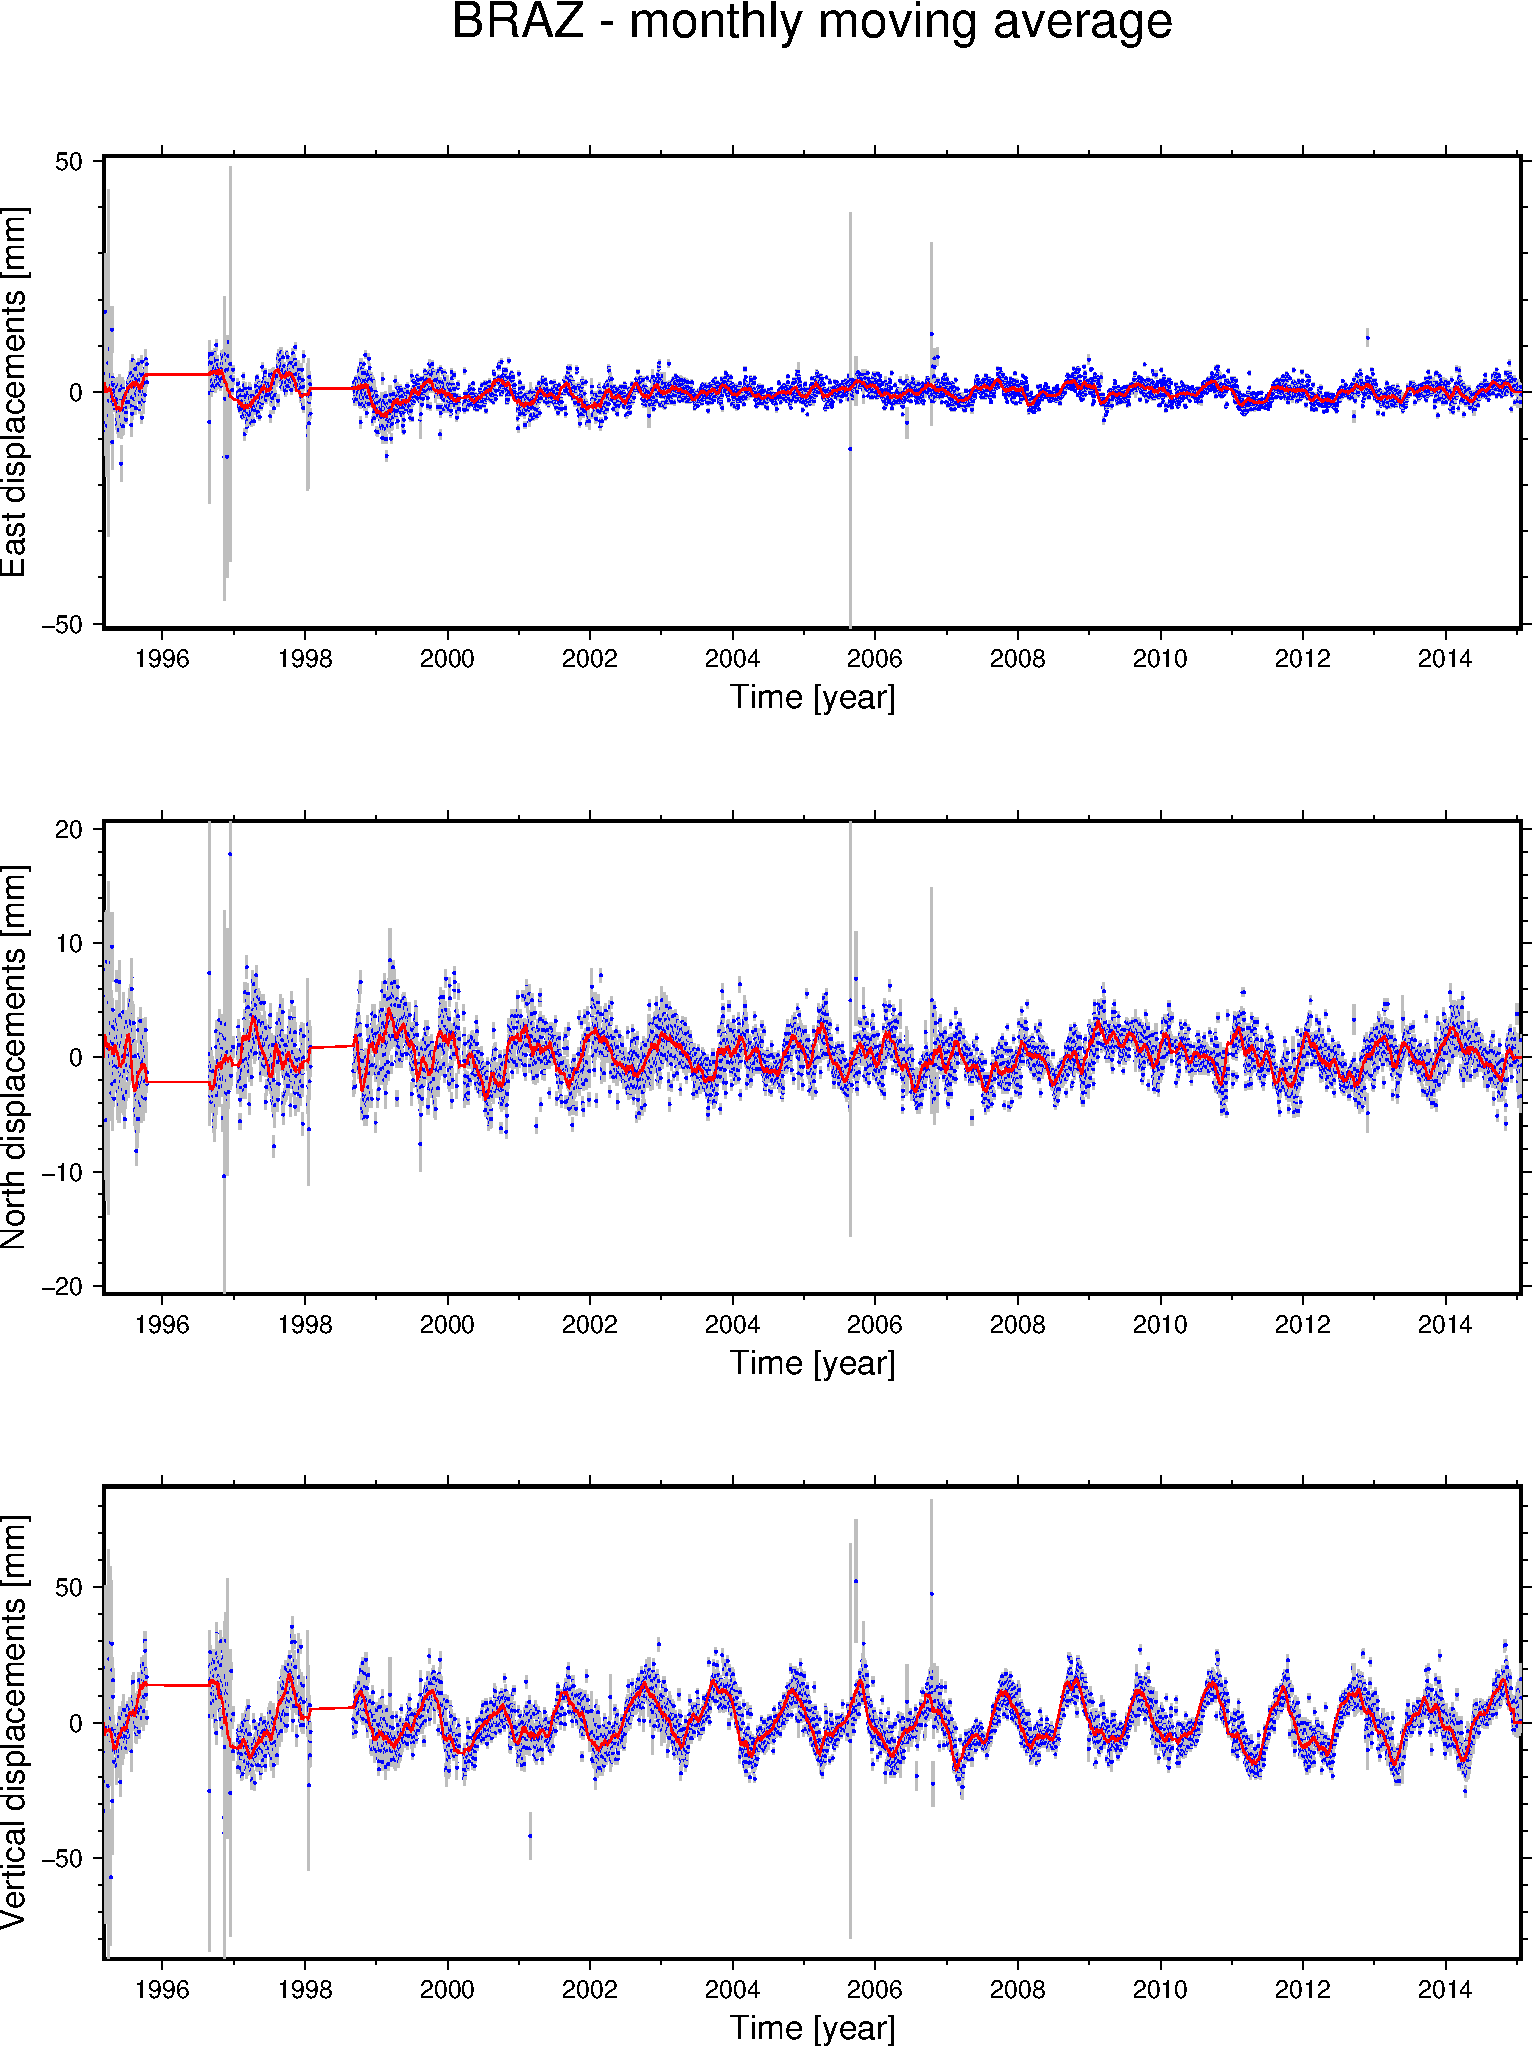
\includegraphics[width=0.40\textwidth]{figures/BRAZ_ma.pdf}
    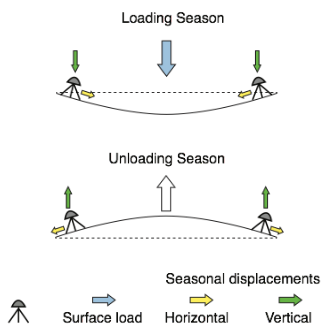
\includegraphics[ width=0.40\textwidth]{figures/schema_gps_load_vertical.png}
        \begin{block}{Question scientifique}
    Dans quelle mesure les modèles de charge expliquent-ils les déplacements mesurés par GNSS ?
    \end{block}
    $\rightarrow$ Jiang et al. (2013) \\ $\rightarrow$ Li et al. (2016)
\end{frame}



\begin{frame}
\frametitle{Plan}
\tableofcontents
\end{frame}


\section{Données}


\begin{frame}
\frametitle{Gravity Recovery And Climate Experiment (GRACE)}

\begin{columns}
        \begin{column}{0.2\textwidth}
        \centering
          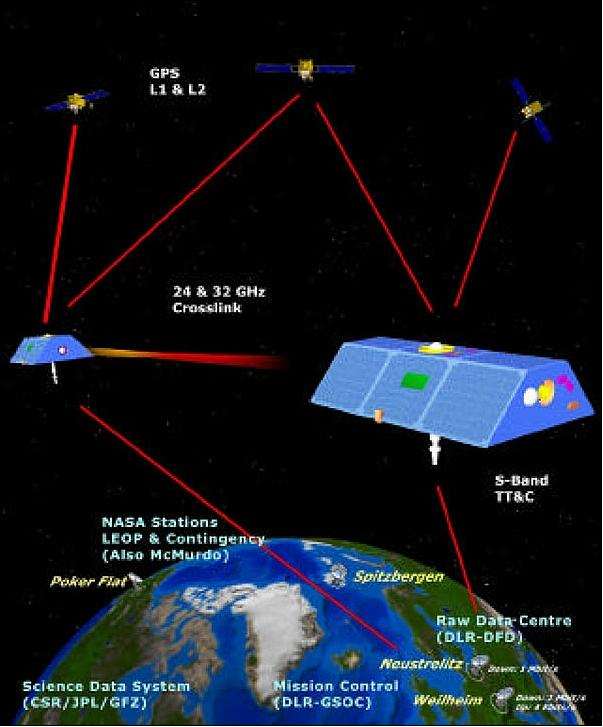
\includegraphics[width=\textwidth]{figures/GRACE_satellites.jpg}
        \end{column}
        \begin{column}{0.8\textwidth}
        \centering
        Hauteur d'eau équivalente saisonnière en mm (2002-2017) \vspace*{-1cm}
          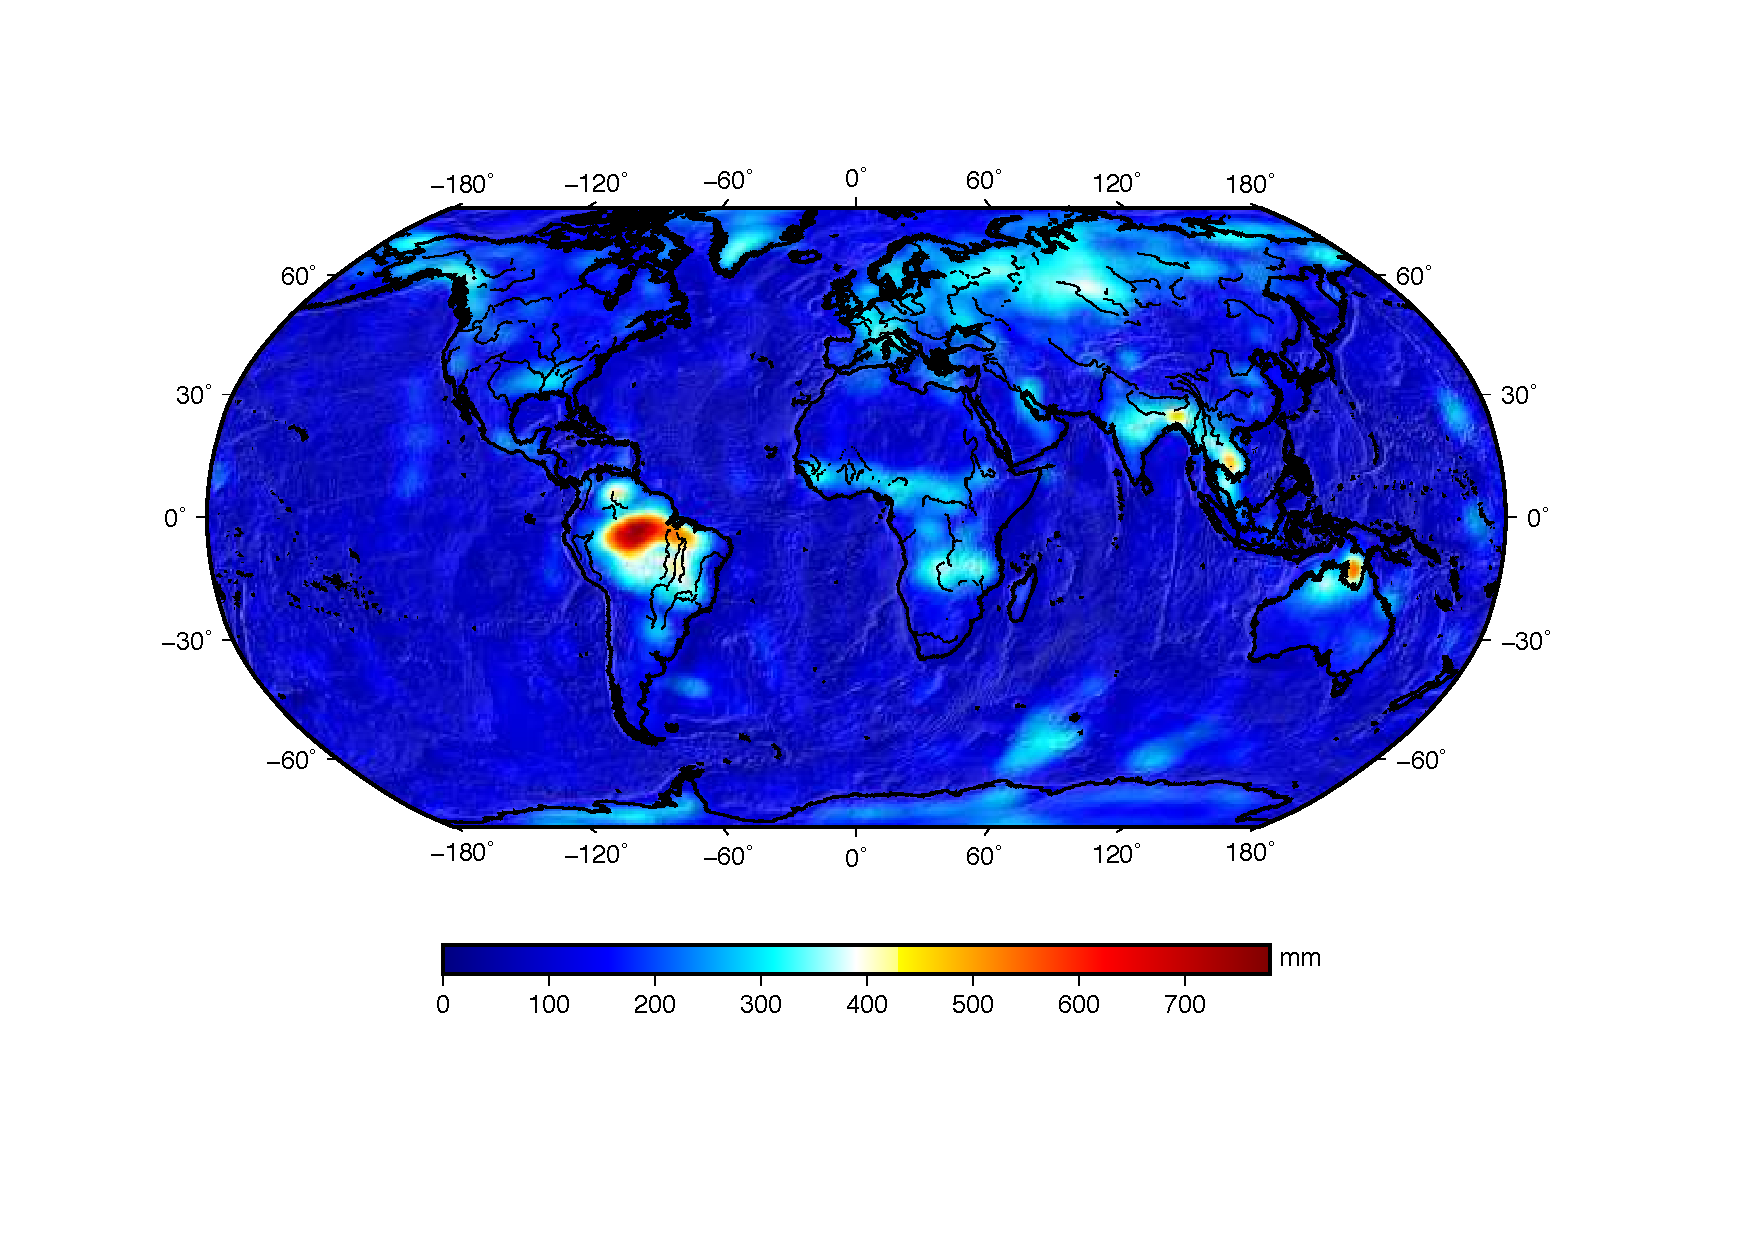
\includegraphics[width=\textwidth]{figures/global_map_grace.pdf} 
          \tiny{\textit{(Chanard et al., 2018)}}
        \end{column}
    \end{columns}
          \begin{itemize}
              \item Mission satellite tandem (2002-2017)
              \item Cartographie des variations spatio-temporelles du champ de gravité
              \item Mesure des redistributions des masses océaniques, atmosphériques et hydrologiques
              \item Résolution: $\sim$400km $\times$ 1 mois
          \end{itemize}
\end{frame}


\begin{frame}
\frametitle{Modèles environnementaux}
\centering
Exemple : \textbf{ECCO}, Estimating the Circulation and Climate of the Ocean\\
    \begin{columns}
        \begin{column}{0.5\textwidth}
            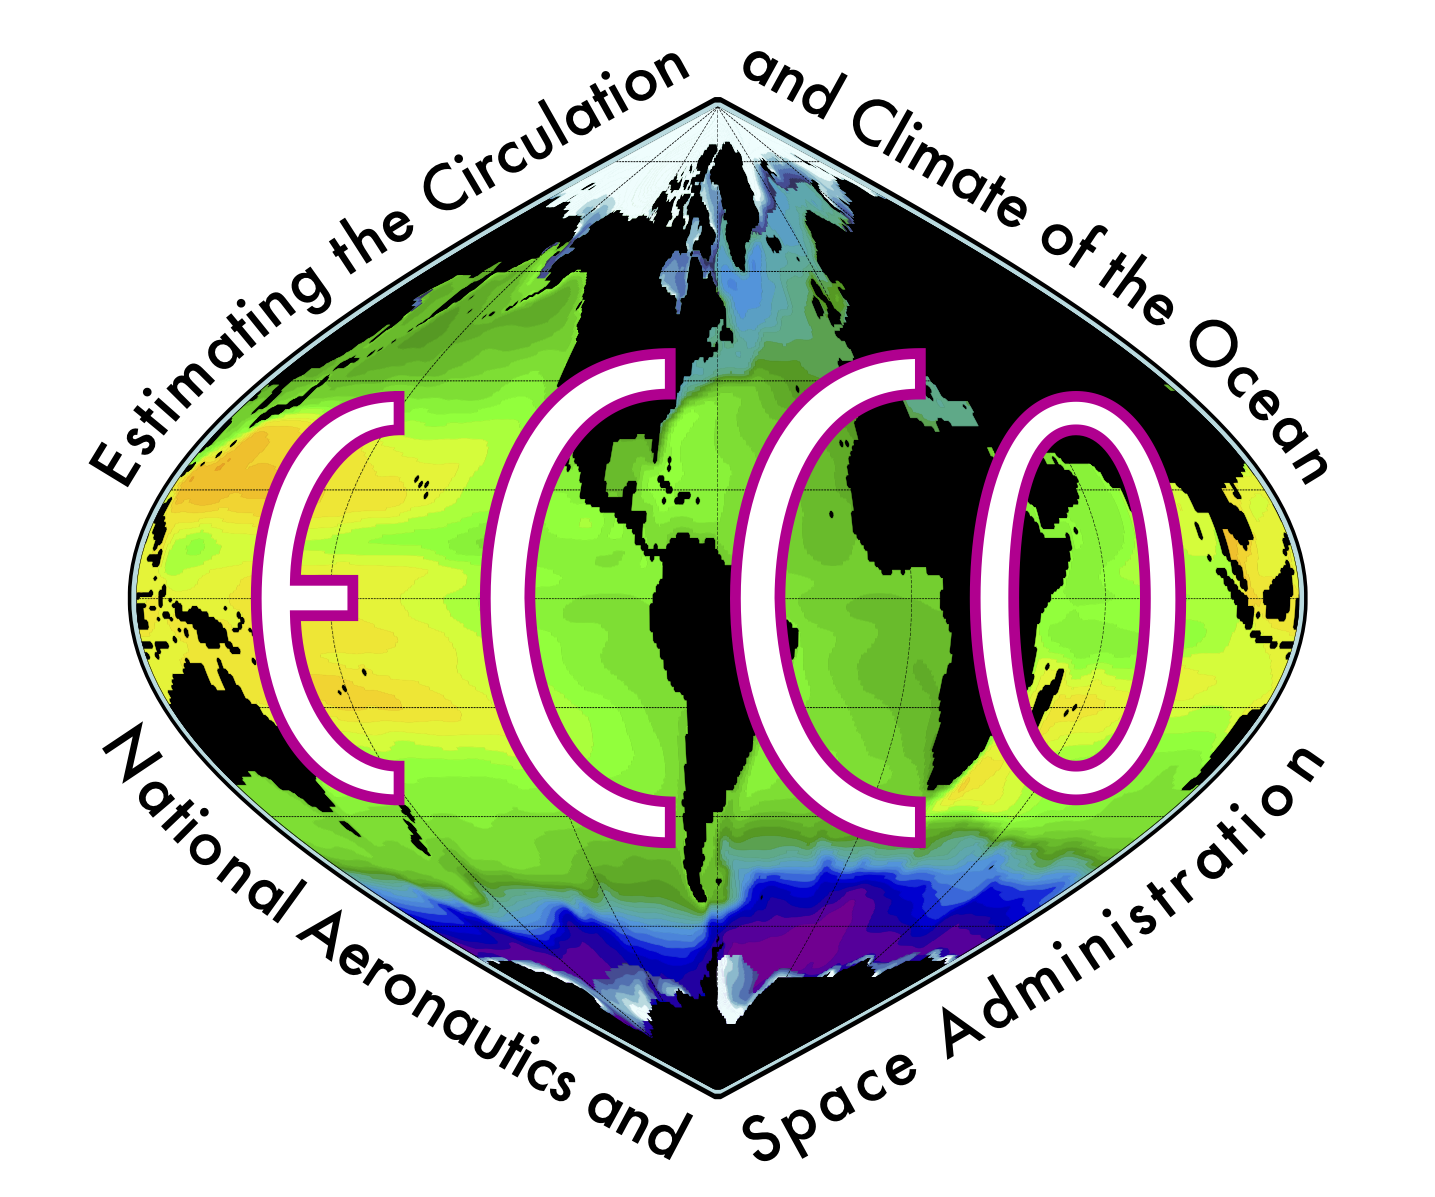
\includegraphics[width=0.7\textwidth]{figures/ecco.png}
            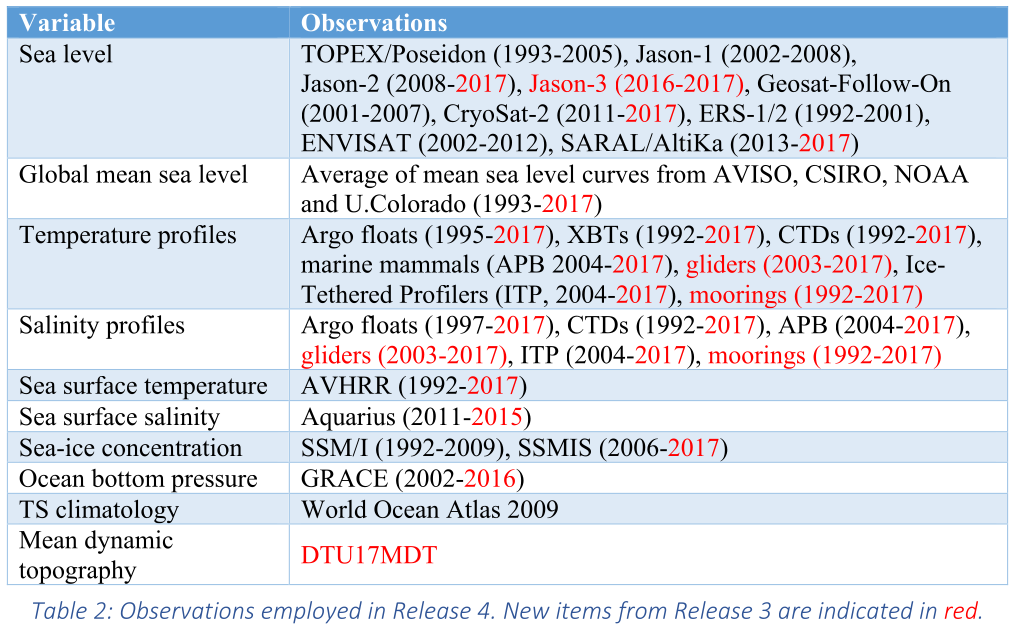
\includegraphics[width=\textwidth]{figures/obs_ecco.png}
        \end{column}
        \begin{column}{0.5\textwidth}
            \centering
            Gliders\\
            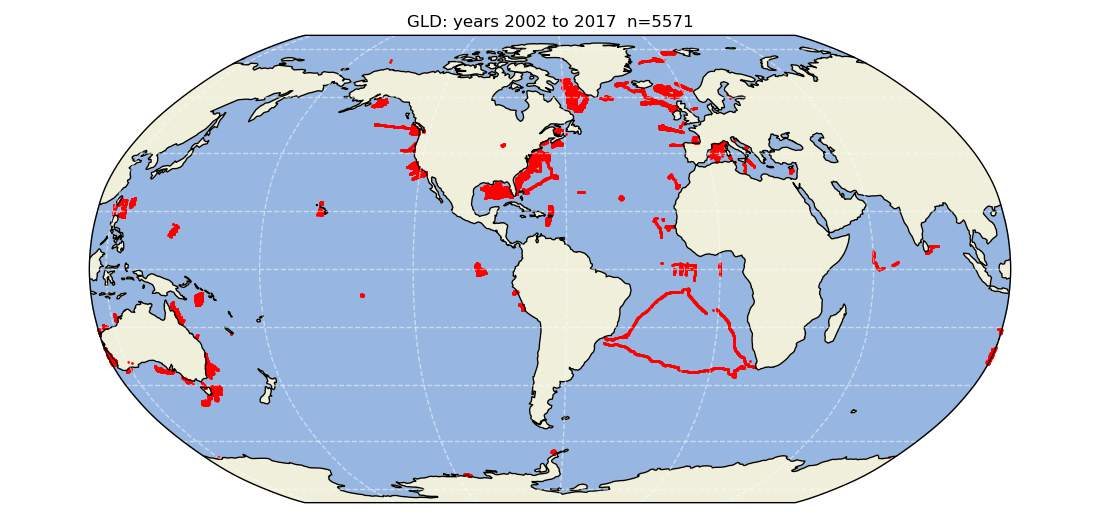
\includegraphics[width=0.7\textwidth]{figures/gliders_distribution.png} \\
            Argos\\
            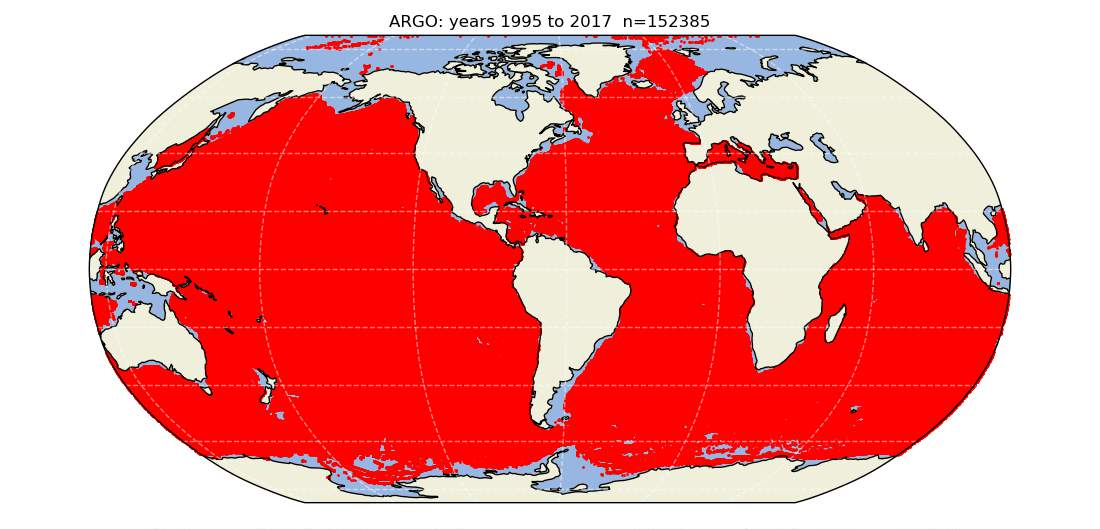
\includegraphics[width=0.7\textwidth]{figures/argos_distribution.png}
            \begin{itemize}
              \item Modèle physique : MIT general circulation model
              \item Prédiction des mouvements de masses océaniques
              \item Résolution: $\sim$100km $\times$ 1 heure/1 jour/1 mois
            \end{itemize}
            
        \end{column}
    \end{columns}
\centering
\begin{workblock}{}
     \small{Travail de conversion : Lat-Lon-Cap 90 $\rightarrow$ grille globale $\rightarrow$ coefficients en harmoniques sphériques.}
\end{workblock}
    
\end{frame}


\section[Déformations de la Terre par...]{Déformations de la Terre par des charges de surface}

\begin{frame}
\frametitle{Prédiction d'un modèle à une station}
\begin{columns}
        \begin{column}{0.6\textwidth}

            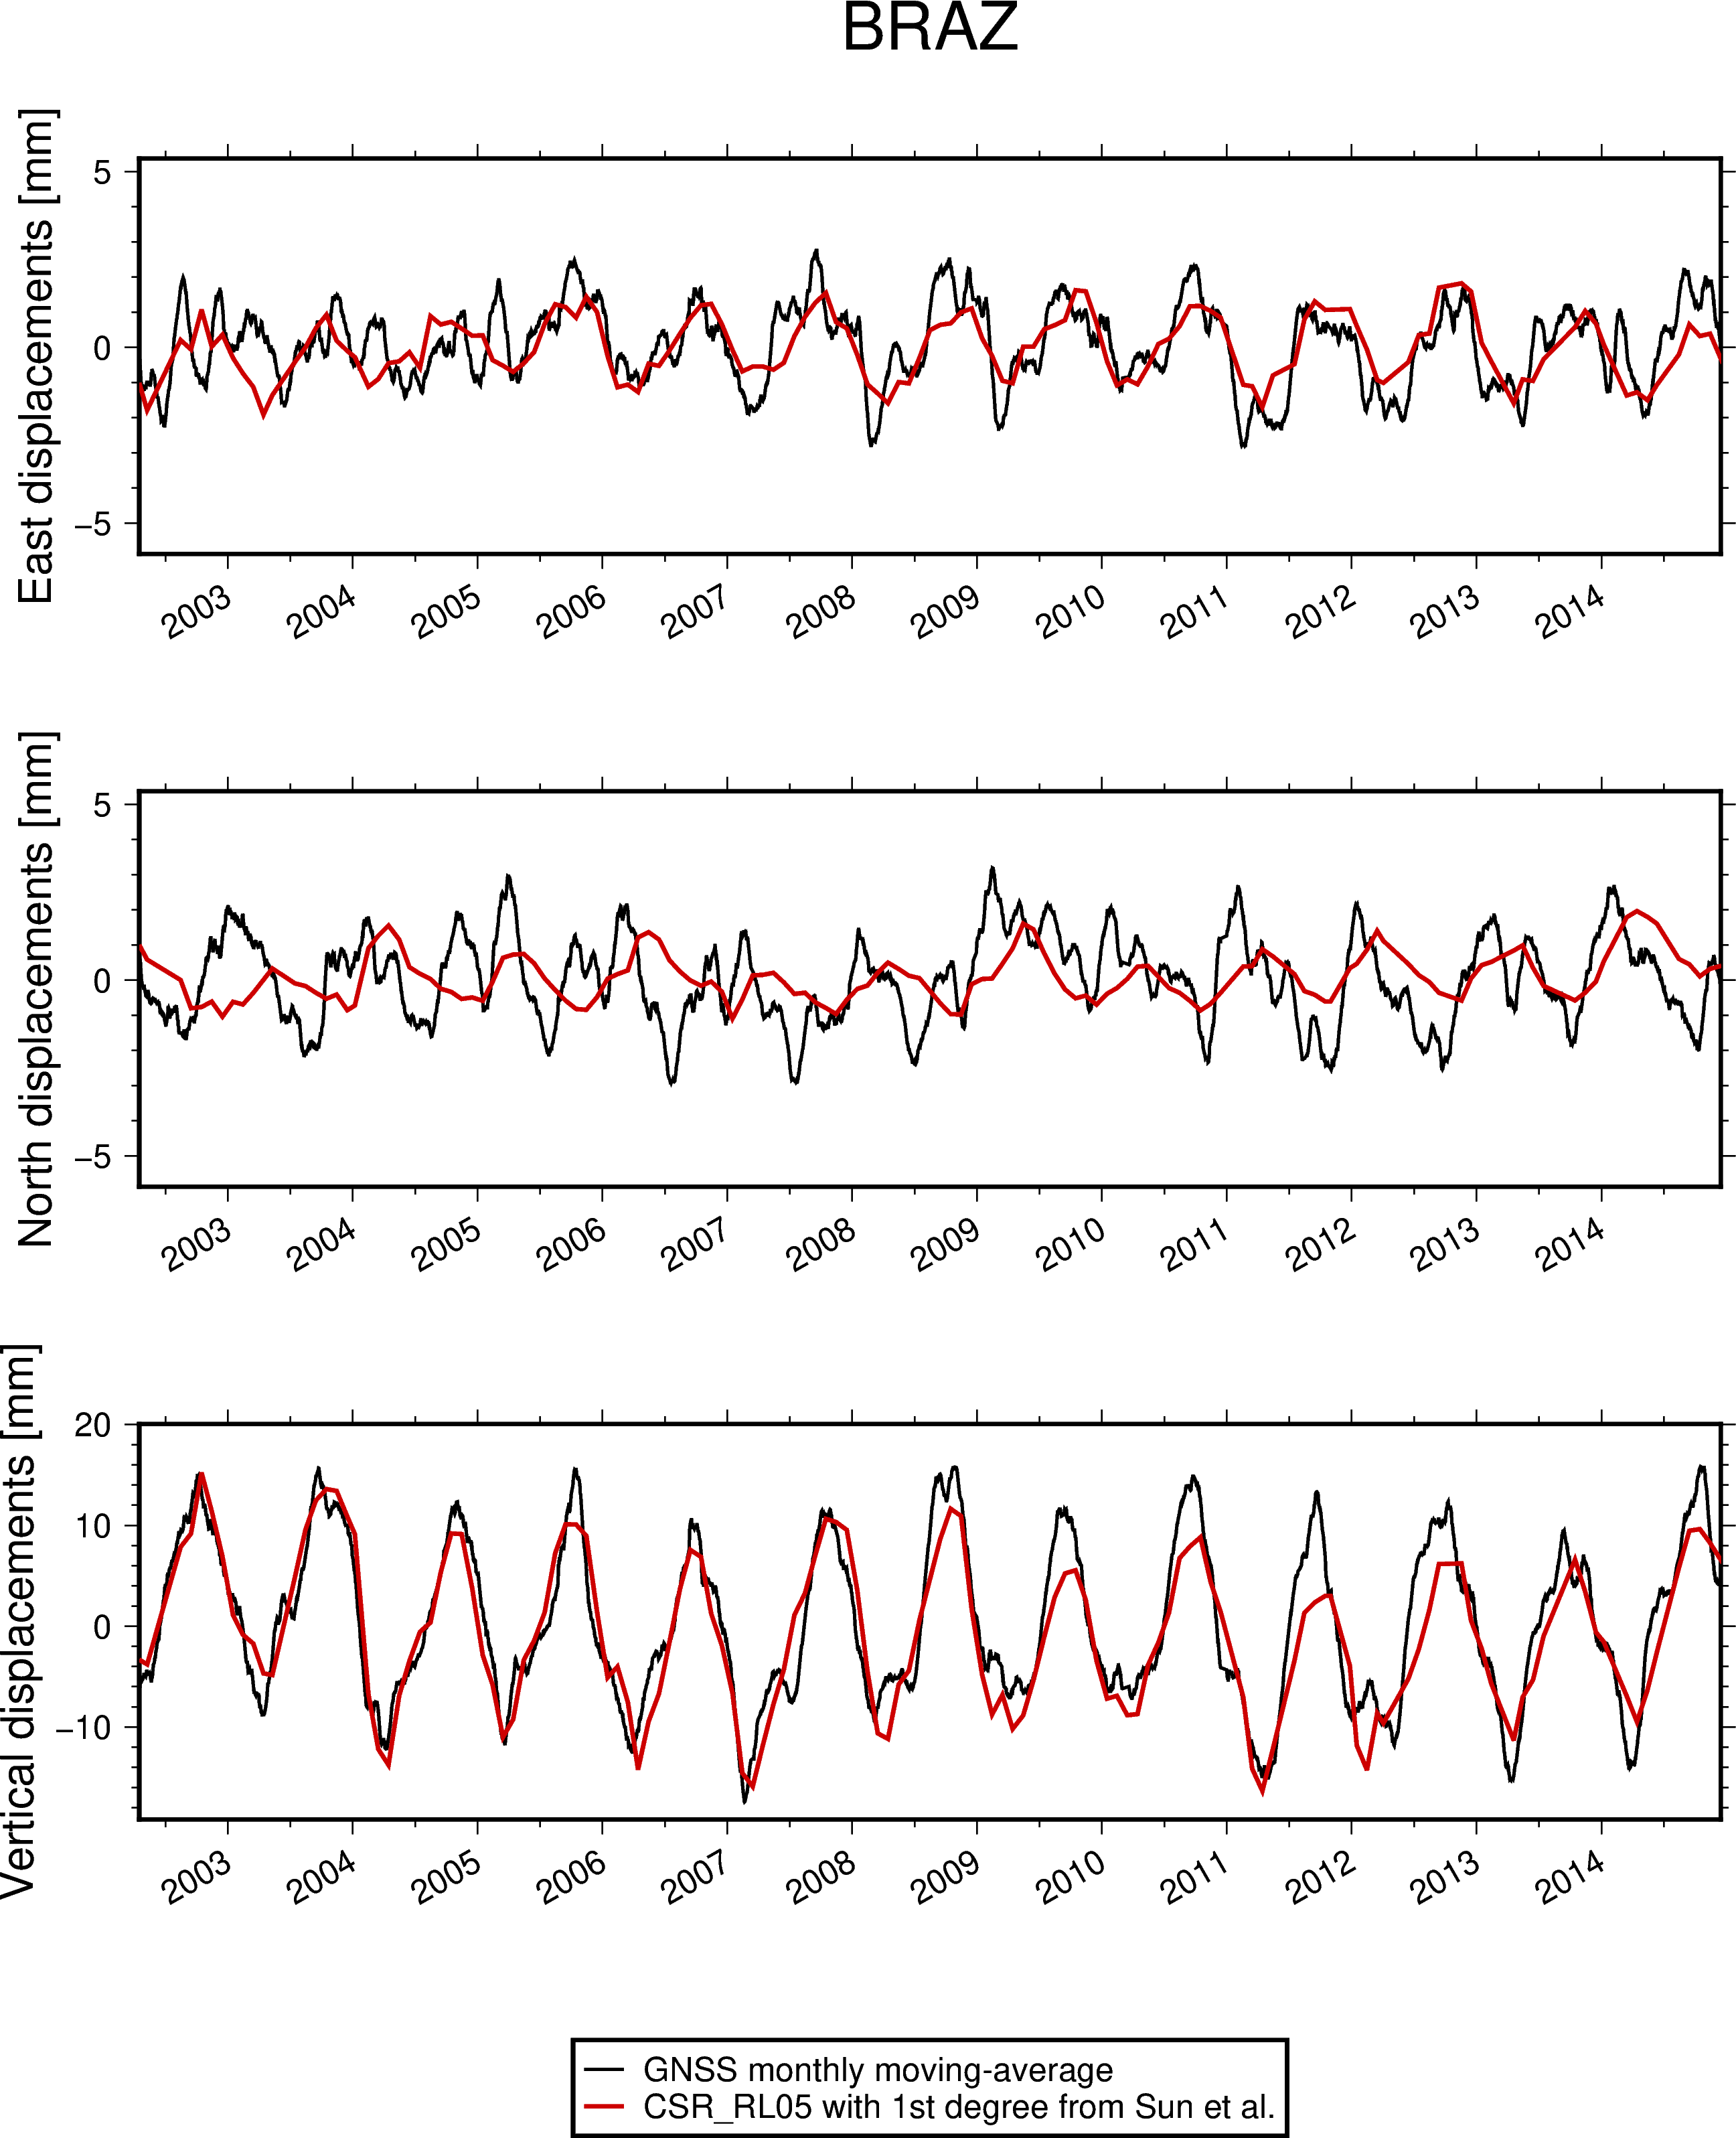
\includegraphics[width=\textwidth]{figures/BRAZ_GRACE_CSR5_w1dSun_vs_IG2.png}
        \end{column}
        \begin{column}{0.45\textwidth}
            \begin{itemize}
                \item Utilisation du degré-1 estimé par Sun et al. (2016) \\(degré-1 non mesuré par GRACE)
                \item Insuffisante sur les composantes planimétriques également vraie sur l'ensemble du réseau
            \end{itemize}   
        \end{column}
\end{columns}


\end{frame}

%\begin{frame}
%\frametitle{Comparaison de modèles}
%Carte de réduction de variance du signal complet (sans séparation annuel/semi-annuel)
%\begin{workblock}{}
% \small{Analyse statistique GNSS-modèles}
%\end{workblock}
%\end{frame}


\section[Particularité des charges de...]{Particularité des charges de très grande longueur d'onde}


\section*{Conclusion}

\begin{frame}
\frametitle{Conclusion}
\begin{block}{Conclusion}
     \begin{itemize}
        \item Préparation et normalisation de nombreux modèles de charge pour le calcul de déformations via ALIEDOCS.
        \item Étude et inversion du degré-1 à partir d'un réseau GNSS et d'un modèle de charges.
        \item Analyse statistique comparée des différents modèles de charges (à suivre...).
\end{itemize}
     \end{block}

\begin{block}{Perspectives}
\begin{itemize}
    \item Expliquer le reste du signal par la déformation thermoélastique du sol et/ou du monument GNSS.
\end{itemize}
\begin{columns}
        \begin{column}{0.6\textwidth}
            \centering
            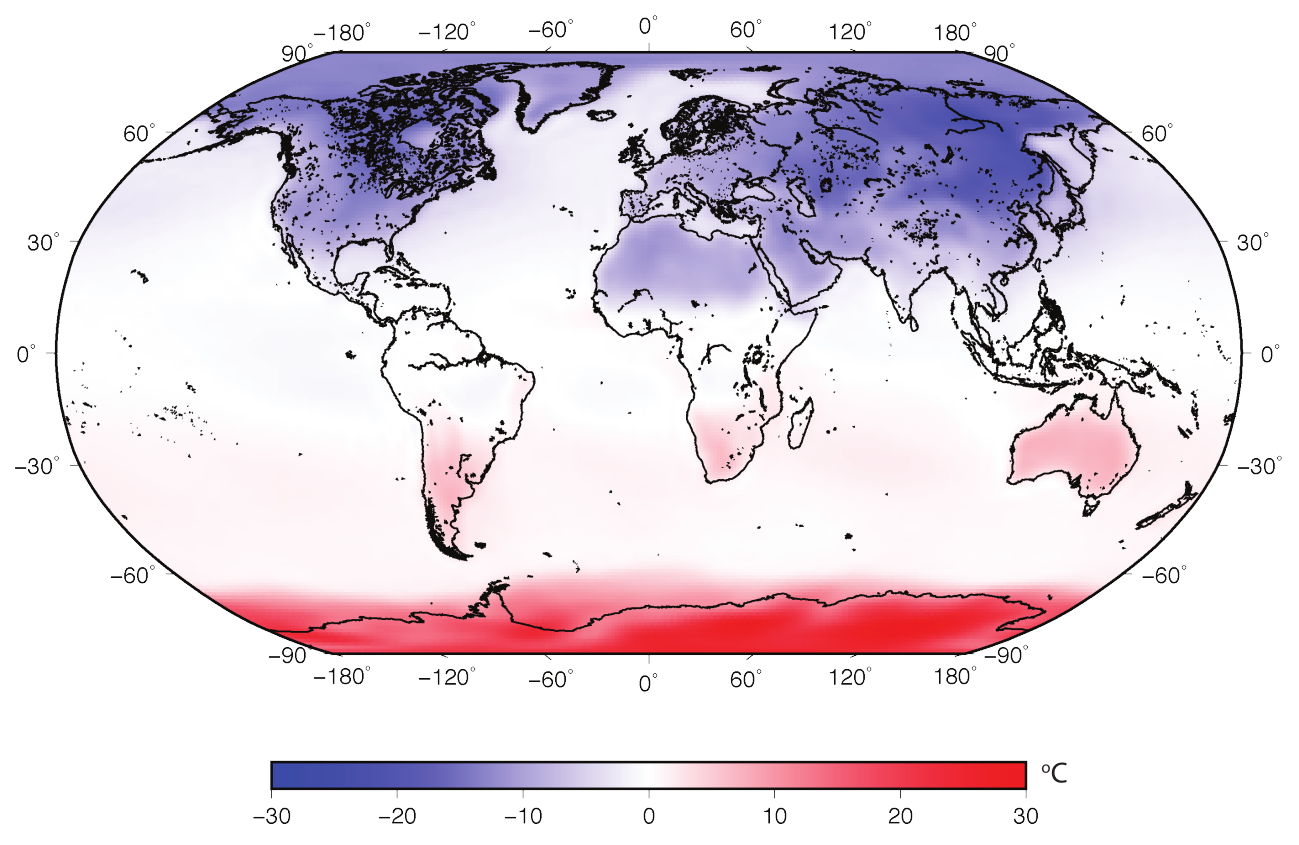
\includegraphics[height=0.26\textheight]{figures/temperature_field.png}
        \end{column}
        \begin{column}{0.4\textwidth}
            \small{Température moyenne en Janvier comparée à la température moyenne annuelle sur la période 2002-2015}
        \end{column}
\end{columns}
\begin{itemize}
    \item Étudier la variabilité de l'inversion du degré-1 en fonction de l'homogénéité du réseau utilisé.
\end{itemize}


\end{block}
\end{frame}

\end{document}

